\documentclass[11pt,a4paper]{article}

\usepackage[T1]{fontenc}
\usepackage[utf8]{inputenc}
\usepackage[french]{babel}
\usepackage{lmodern}
\usepackage{amsmath,amssymb}
\usepackage{graphicx}
\usepackage{booktabs}
\usepackage{microtype}
\usepackage[margin=2.4cm]{geometry}
\usepackage[hidelinks]{hyperref}
\usepackage{natbib}
\bibliographystyle{plainnat}

\graphicspath{{figures/}}

\title{\textbf{De la décohérence quantique à la polarisation sociale}\\[2mm]
       \large Modélisation thermodynamique de l'opinion publique\\
       et proposition d'un index métrologique}
\author{Sylvain Geffroy}
\date{Août 2026 --- \emph{document de travail ouvert à la relecture}}

\begin{document}
\maketitle

\begin{abstract}
\noindent
Plus un système quantique est grand, plus sa décohérence est rapide. Plus une population
est grande, plus il est difficile d'y trouver un accord. Cette note formalise l'analogie
structurelle entre ces deux phénomènes et en teste les conséquences numériquement.

Avec l'énergie libre de Helmholtz $F = E - TS$ écrite complètement, la distribution
stationnaire des opinions présente une \emph{transition de phase} : au-dessus d'une
température sociale critique, un pic unique centré sur la modération ; en dessous, deux
pics extrêmes. Sous cette température, l'effacement du champ médiatique ne restaure pas
la neutralité --- le conformisme de groupe entretient une \emph{hystérésis}, ce qui
explique l'inefficacité du démenti passif. Enfin, lorsque le gain algorithmique excède le
taux d'amortissement naturel d'un contenu ($\gamma\alpha > \lambda$), l'amortissement
effectif devient négatif et le système entre en résonance --- un effet Larsen
informationnel.

Nous en dérivons deux instruments : l'\textbf{Index de Dissipation Entropique} (IDE),
métrique auditable de la diversité informationnelle d'un fil, et l'\textbf{Algorithme de
Dissipation Entropique} (ADE), filtre de recommandation qui optimise cet index plutôt que
l'engagement brut.

Une calibration sur des séries d'attention publiques (\S\ref{sec:calibration}) situe le
rapport $\gamma\alpha/\lambda$ entre $1{,}5$ et $12$ sur dix-neuf épisodes. Elle montre du
même coup que le critère d'instabilité est satisfait par construction pour tout épisode
observable : sa vérification n'apprend rien, et la recommandation réglementaire
correspondante doit porter sur un plafond du rapport.

La section~\ref{sec:limites} énonce les limites du travail. L'intégralité du code, des
tests et des figures est reproductible en conteneur.
\end{abstract}

\section{Introduction et hypothèse}

La sociophysique applique depuis les années 1980 les outils de la physique statistique à
la dynamique d'opinion \citep{galam2004,castellano2009}. Cette note part d'une observation
plus étroite et plus précise.

En physique quantique, un système isolé existe dans une superposition d'états. Au contact
d'un environnement, il s'intrique avec lui et les termes d'interférence
s'annulent~: c'est la décohérence \citep{zeh1970,zurek2003}. Plus l'environnement est
massif, plus le phénomène est rapide.

L'hypothèse de travail est la suivante :

\begin{quote}
L'augmentation de la taille d'un système ($N \to \infty$) détruit la cohérence de son état
initial --- en physique quantique en accélérant la décohérence, en dynamique d'opinion en
rendant le consensus organique inatteignable.
\end{quote}

Cette hypothèse est \emph{structurelle} : elle affirme qu'un même formalisme décrit les
deux situations, non que les opinions humaines obéissent à des lois physiques. Sa valeur
tient à ce qu'elle produit des quantités mesurables. Nous verrons cependant
(\S\ref{sec:limites}) qu'elle demande une reformulation importante : l'effet de $N$ n'est
pas d'ajouter du désordre, mais de retirer de la plasticité.

\section{Formalisme entropique}

\subsection{Deux entropies, une même grandeur}

L'entropie de von Neumann \citep{vonneumann1932}
\begin{equation}
S(\rho) = -\operatorname{Tr}(\rho \ln \rho)
\end{equation}
est nulle pour un état pur. Son calcul passe par diagonalisation : les valeurs propres de
$\rho$ forment une distribution classique à laquelle on applique l'entropie de Shannon
\citep{shannon1948}
\begin{equation}
H(X) = -\sum_i p_i \log_2 p_i .
\end{equation}
C'est précisément ce qui autorise le pont entre les deux disciplines : l'entropie de von
Neumann \emph{est} l'entropie de Shannon du mélange révélé par la base propre.

\subsection{Une précision nécessaire}

Il faut écarter d'emblée une formulation courante et fausse. L'évolution d'un système
quantique \emph{fermé} est unitaire, donc son entropie de von Neumann est constante. Ce
qui croît sous l'effet de la décohérence est l'entropie du \emph{sous-système réduit},
obtenue en traçant sur les degrés de liberté de l'environnement.

Il en découle une clarification qui renforce l'analogie plutôt qu'elle ne l'affaiblit :
une superposition cohérente est un état \emph{pur}, d'entropie nulle. Ce n'est donc pas la
multiplicité des possibilités qui produit du désordre, mais la perte de cohérence entre
elles. Le pendant social est plus juste ainsi : une population où chacun garde plusieurs
opinions ouvertes n'est pas désordonnée --- le désordre naît du contact avec un
environnement qui fixe les positions.

\section{Dynamique thermodynamique}

\subsection{Modèle d'Ising et température sociale}

Chaque individu porte une opinion binaire $s_i \in \{-1,+1\}$ et la population suit la
distribution de Gibbs-Boltzmann \citep{ising1925} :
\begin{equation}
P(\sigma) = \frac{1}{Z}
\exp\!\left(\frac{J \sum_{\langle i,j\rangle} s_i s_j + H \sum_i s_i}{k_B T}\right),
\end{equation}
où $J$ mesure la force de conformisme local, $T$ la \emph{température sociale} (agitation,
irrationalité, ouverture aux fluctuations) et $H$ le champ médiatique externe.

L'intérêt du modèle ne réside pas dans l'analogie mais dans une propriété vérifiable :
l'existence d'une température critique. En dimension deux, sa valeur exacte est connue
\citep{onsager1944} :
\begin{equation}
\frac{T_c}{J} = \frac{2}{\ln(1+\sqrt{2})} \approx 2{,}269 .
\label{eq:onsager}
\end{equation}

C'est le seul point de ce travail où une prédiction théorique exacte, indépendante de nos
hypothèses sociologiques, peut valider l'implémentation. La figure~\ref{fig:transition} la
retrouve numériquement ; l'écart résiduel s'explique par les effets de taille finie sur un
réseau de $24\times24$.

\begin{figure}[t]
\centering
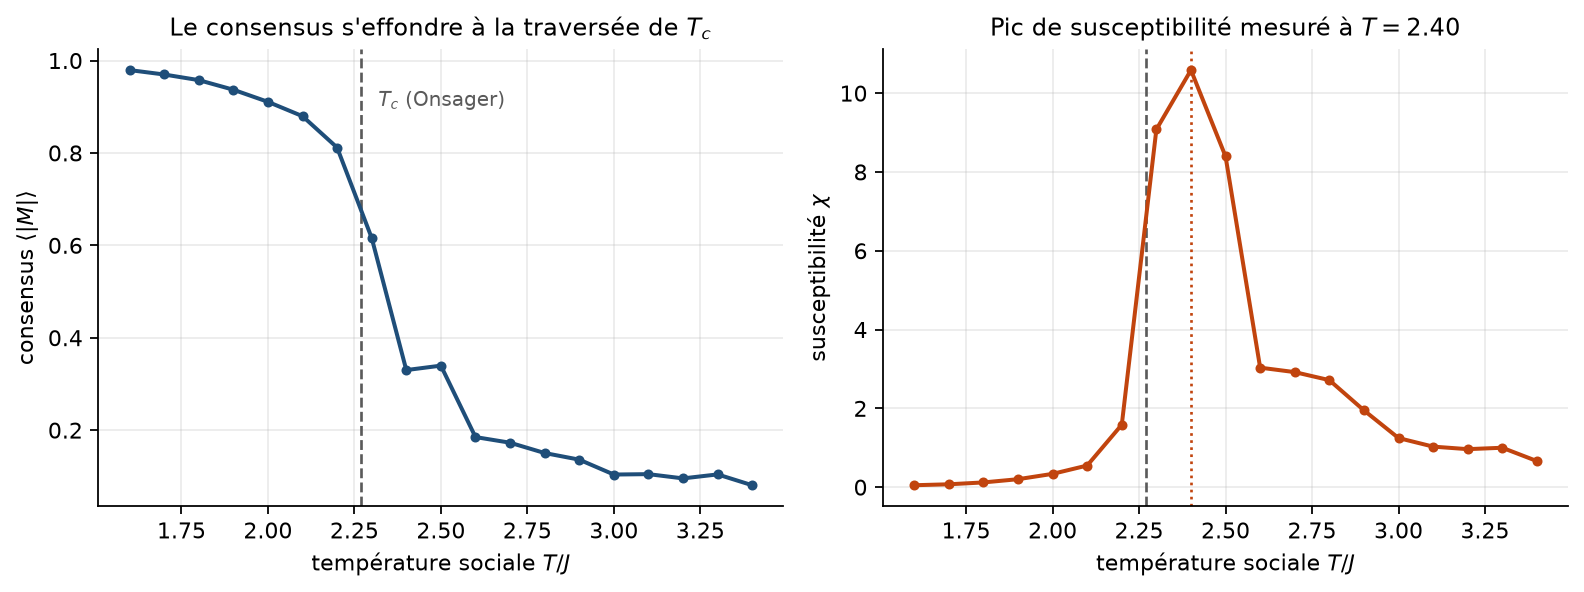
\includegraphics[width=\linewidth]{fig02_transition.png}
\caption{Consensus et susceptibilité en fonction de la température sociale (Monte-Carlo,
réseau $24\times 24$). Le pic de susceptibilité localise la transition. Le décalage vers
le haut par rapport à la valeur d'Onsager~\eqref{eq:onsager} est un effet de taille finie,
non une erreur d'implémentation.}
\label{fig:transition}
\end{figure}

\subsection{Énergie libre}

Le système minimise son énergie libre de Helmholtz $F = E - TS$, où $E$ représente la
tension du désaccord et $TS$ la force de dispersion. Quand $N$ croît, l'entropie de
configuration croît avec elle et le terme $TS$ finit par dominer $E$.

\subsection{Hystérésis sociale}

C'est le résultat le plus directement actionnable. Sous $T_c$, couper le champ médiatique
($H \to 0$) ne ramène pas l'aimantation à zéro : le terme d'interaction
$-J\sum s_i s_j$ prend le relais et le groupe maintient la croyance par cohésion interne.

Le cycle se lit en trois temps, qui sont ceux d'une crise médiatique : injection d'un champ
massif, démenti officiel, puis nécessité d'un contre-champ $-H$ dépassant le champ
coercitif du groupe. La figure~\ref{fig:hysteresis} montre que l'aire du cycle décroît
avec la température sociale et s'annule au-dessus de $T_c$.

\begin{figure}[t]
\centering
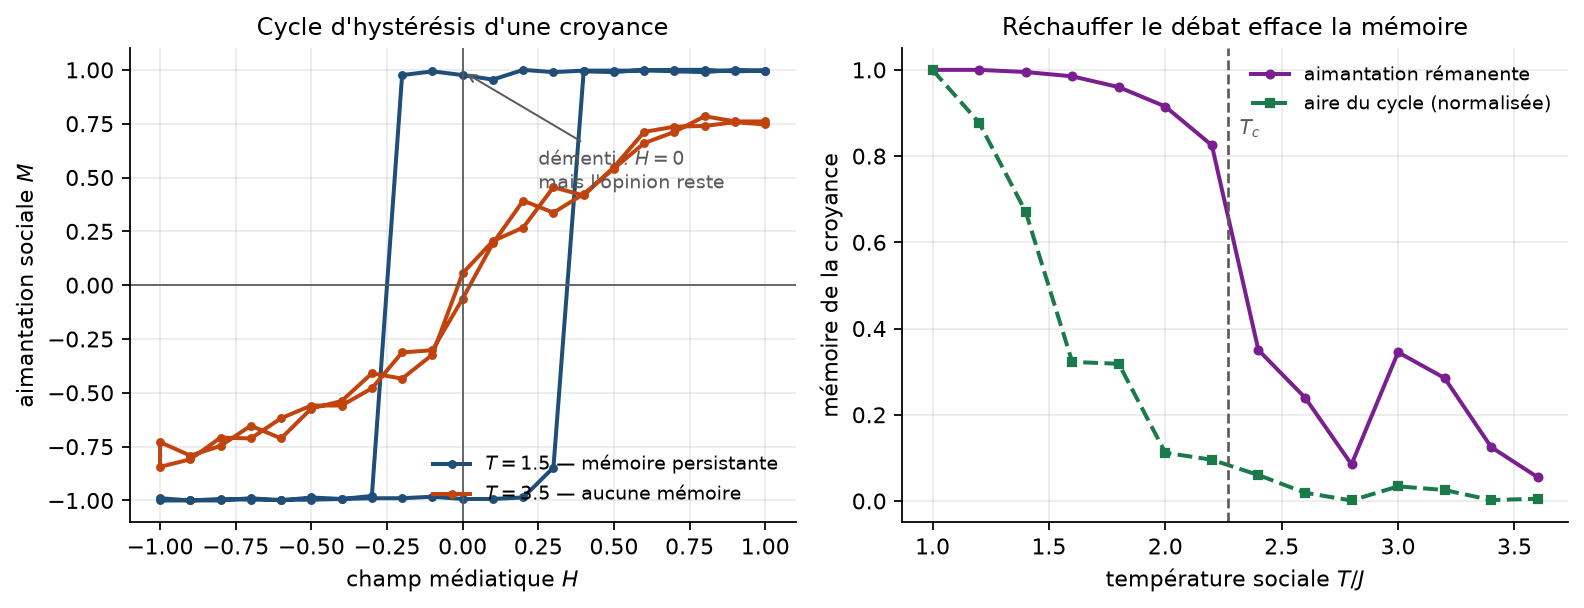
\includegraphics[width=\linewidth]{fig05_hysteresis.png}
\caption{À gauche, cycles d'hystérésis sous et au-dessus de $T_c$ : dans le premier cas
l'opinion reste aimantée alors que le champ est nul. À droite, décroissance de la mémoire
avec la température sociale --- fondement de la recommandation d'injection de bruit.}
\label{fig:hysteresis}
\end{figure}

\emph{Conséquence pratique :} le \emph{debunking} passif ne fonctionne pas. Rétablir la
neutralité informationnelle laisse la croyance en place ; seule une contre-information
active, ou une hausse de la température sociale, la dissipe.

\section{Effet de taille : temps de consensus}

Le Voter Model \citep{clifford1973,holley1975} isole la contagion sociale pure, sans
température : à chaque interaction un individu adopte l'opinion d'un voisin tiré au hasard.
Il fournit des lois d'échelle exactes pour le temps de consensus, mesuré en balayages
($N$ interactions élémentaires).

Les mesures (figure~\ref{fig:consensus}) donnent un exposant $\approx 1$ en champ moyen et
$\approx 2$ sur un anneau. \textbf{Un réseau densément connecté converge donc plus vite
qu'un voisinage géographique.}

Cette observation infirme un argument fréquent, selon lequel la structure « petit monde »
des réseaux sociaux \citep{watts1998} empêcherait le consensus. La connectivité ne
fragmente pas : elle accélère et amplifie, dans la direction que le champ lui donne. Les
causes de la fragmentation sont le \emph{biais directionnel} des micro-champs
algorithmiques et l'\emph{homophilie} qui compartimente le graphe \citep{pariser2011}. La
conséquence pour la régulation est nette : le levier utile porte sur le champ, non sur le
nombre de liens.

\begin{figure}[t]
\centering
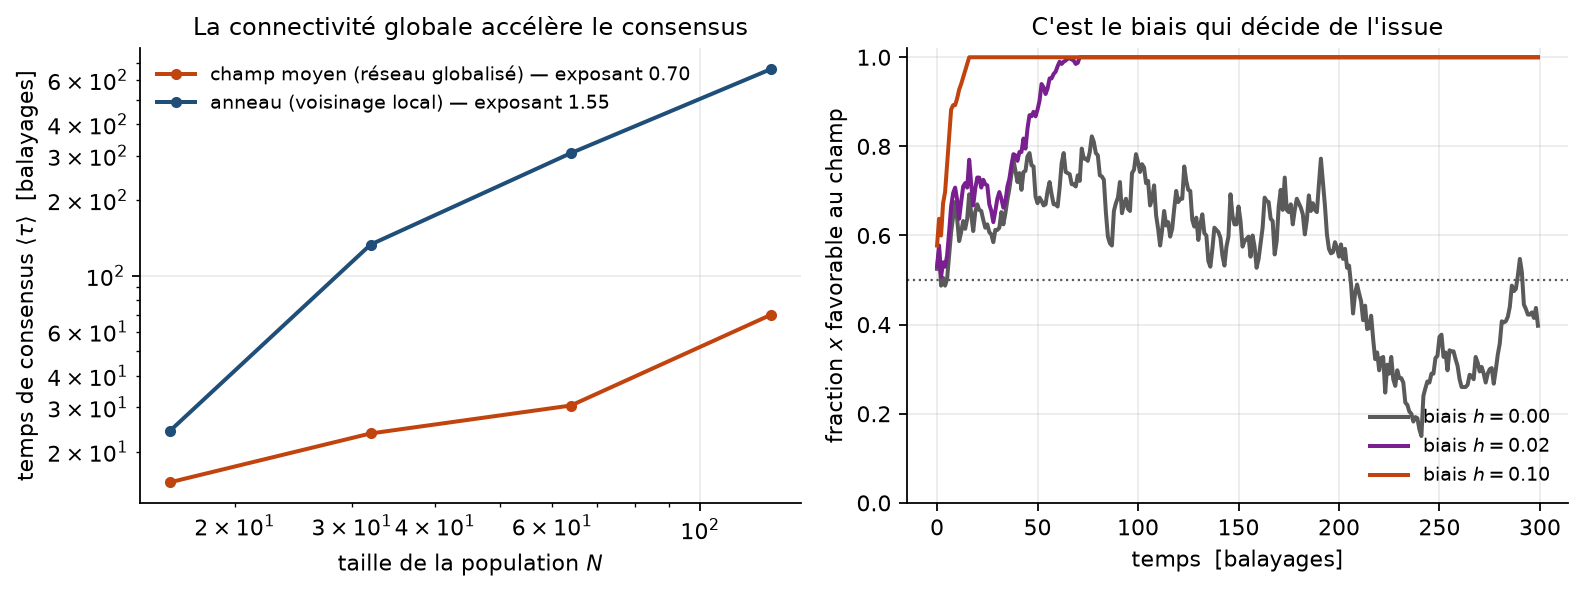
\includegraphics[width=\linewidth]{fig03_consensus.png}
\caption{À gauche, temps de consensus en fonction de la taille de la population, en échelle
log-log, pour deux topologies. À droite, trajectoires de la fraction favorable au champ
pour trois intensités de biais : c'est le biais, non la connectivité, qui décide de
l'issue.}
\label{fig:consensus}
\end{figure}

\section{Paysage de l'opinion publique}

\subsection{L'équation et sa dérive}

À l'échelle macroscopique, l'opinion collective $x \in [-1,1]$ obéit à une équation de
Fokker-Planck \citep{risken1989} :
\begin{equation}
\frac{\partial P(x,t)}{\partial t}
= -\frac{\partial}{\partial x}\big[A(x)P(x,t)\big]
+ \frac{\partial^2}{\partial x^2}\big[B(x)P(x,t)\big].
\end{equation}

Le potentiel quadratique $V(x) = -\frac{J}{2}x^2 - Hx$, qui vient naturellement à l'esprit,
ne peut produire \emph{aucune} transition de phase : l'exponentielle correspondante est
convexe, donc maximale aux extrêmes à toute température. Le terme manquant est l'entropie
de mélange, c'est-à-dire le nombre de configurations individuelles compatibles avec une
opinion moyenne $x$. En l'ajoutant, on retrouve l'énergie libre de Helmholtz :
\begin{equation}
f(x) = \underbrace{-\frac{J}{2}x^2 - Hx}_{E}
+ T\underbrace{\left[\frac{1+x}{2}\ln\frac{1+x}{2}
+ \frac{1-x}{2}\ln\frac{1-x}{2}\right]}_{-S},
\label{eq:libre}
\end{equation}
d'où la dérive
\begin{equation}
A(x) = -f'(x) = Jx + H - T\operatorname{artanh}(x).
\label{eq:derive}
\end{equation}
Le rappel entropique $-T\operatorname{artanh}(x)$ borne la dynamique dans $(-1,1)$ et fait
apparaître une température critique de champ moyen $T_c = J$. La forme $A(x) = Jx + H$ en
est la linéarisation au voisinage de $x = 0$.

\subsection{La diffusion et l'effet de $N$}

Le terme de diffusion s'écrit
\begin{equation}
B(x) = \frac{k_B T (1-x^2)}{N},
\label{eq:diffusion}
\end{equation}
le facteur $(1-x^2)$ éteignant le bruit à l'unanimité.

Le facteur $1/N$ demande une lecture attentive, car il paraît contredire l'hypothèse de
départ : plus la population est grande, \emph{moins} sa variable macroscopique est bruitée.
Il n'y a pas de contradiction, mais deux échelles distinctes. L'entropie de configuration
totale est extensive et croît comme $N$ ; les fluctuations de la moyenne $x$ décroissent en
$1/N$. La thèse défendable est donc :

\begin{quote}
Une grande population ne devient pas bruyante, elle devient \emph{rigide}. Sa taille ne
l'agite pas, elle la prive de plasticité stochastique --- et c'est cette rigidité qui rend
la polarisation irréversible, un système sans bruit ne pouvant plus quitter le puits de
potentiel où il est tombé.
\end{quote}

Cette reformulation est plus forte que l'hypothèse initiale : elle explique
l'irréversibilité, ce que la métaphore de la « pompe à entropie » ne faisait pas.

\subsection{Trois régimes}

La distribution d'équilibre prend la forme de grandes déviations
$P_{\mathrm{stat}}(x) \propto \exp(-N f(x)/T)$, où le facteur $N$ rend la pénalité
d'autant plus sévère que la population est grande. Trois régimes en découlent, obtenus en
faisant varier deux paramètres (figure~\ref{fig:paysage}) : société fluide ($T > T_c$),
polarisée ($T < T_c$, $H = 0$) et manipulée ($T < T_c$, $H > 0$). Dans le dernier cas, le
pic situé du côté du champ écrase l'autre : le « faux consensus » n'est pas une hypothèse
ajoutée, c'est le puits incliné.

La densité de modérés décroît exponentiellement avec $N$. Dans une grande population sous
$T_c$, la modération n'est pas minoritaire : elle est statistiquement inaccessible.

\begin{figure}[t]
\centering
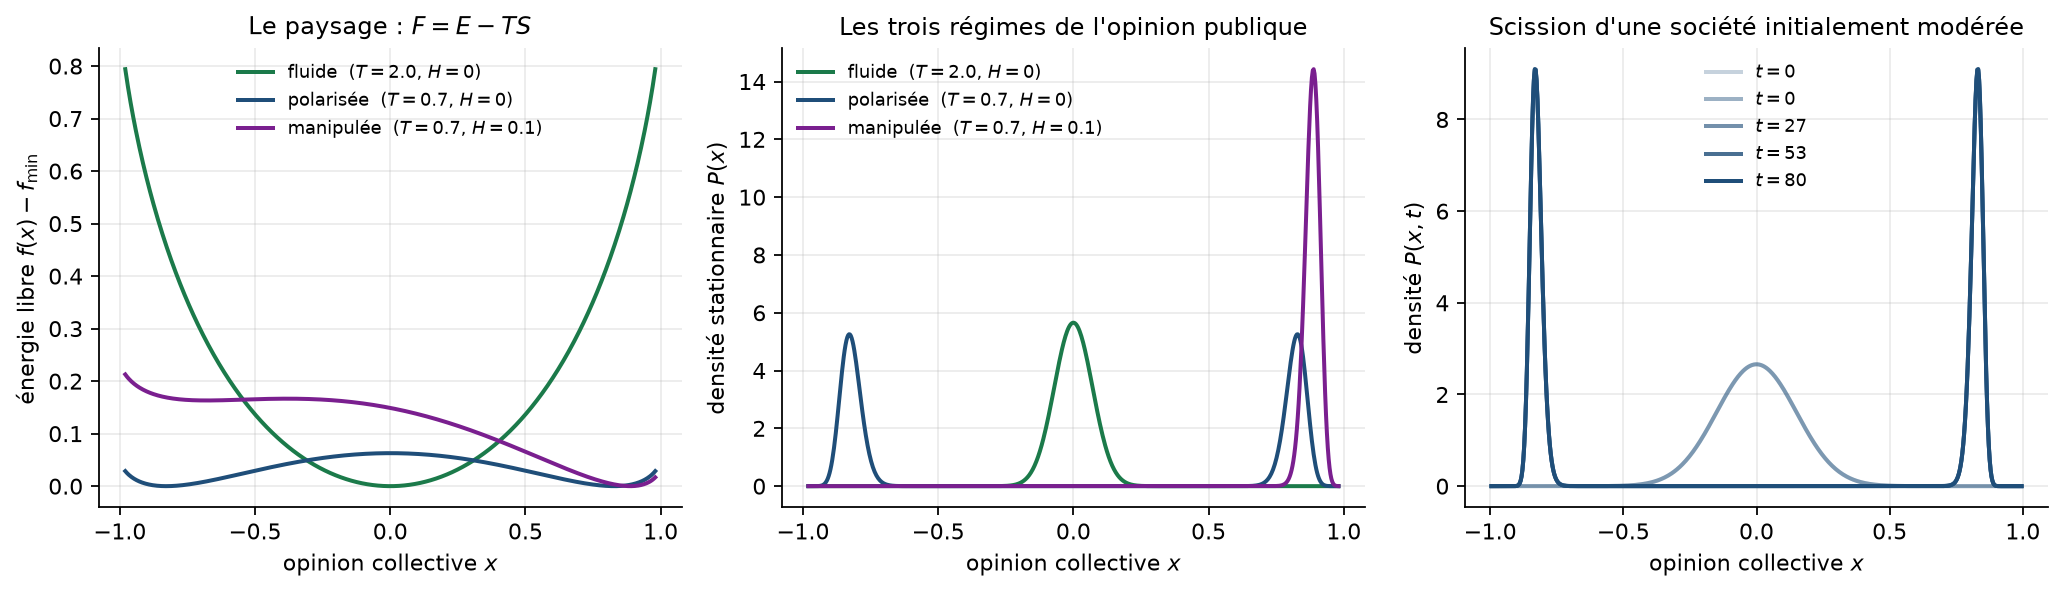
\includegraphics[width=\linewidth]{fig04_paysage.png}
\caption{Paysage d'énergie libre~\eqref{eq:libre}, distributions stationnaires associées et
scission temporelle d'une société initialement modérée. Le solveur est en volumes finis à
flux nul aux bords : la masse de probabilité est conservée à $10^{-15}$, ce qui distingue un
effondrement réel de la modération d'une fuite numérique.}
\label{fig:paysage}
\end{figure}

\subsection{Franchissement de barrière}

Le passage d'un bloc à l'autre sans traverser la modération relève du franchissement de
barrière par activation thermique, de taux $\propto e^{-\Delta V / k_B T}$
\citep{kramers1940}, et non d'un effet tunnel --- lequel n'a pas d'équivalent classique. La
distinction n'est pas cosmétique : la loi de Kramers fournit une dépendance en température
donc une prédiction testable.

\section{Cinétique de résonance algorithmique}

Une fausse information et un algorithme de recommandation forment une boucle de rétroaction
positive analogue à l'effet Larsen. La visibilité $V(t)$ obéit à
\begin{equation}
\ddot V + \big(\lambda - \gamma\alpha\,\sigma(V)\big)\dot V + \omega_0^2 V = \xi(t),
\label{eq:resonance}
\end{equation}
où $\lambda$ est l'amortissement naturel (l'oubli), $\gamma$ le gain algorithmique,
$\alpha$ la charge émotionnelle du contenu, et $\sigma(V) = 1/(1+(V/V_{\mathrm{sat}})^2)$
un facteur de saturation traduisant la finitude de l'attention disponible.

Le critère d'instabilité est
\begin{equation}
\boxed{\;\gamma\alpha > \lambda\;}
\label{eq:critere}
\end{equation}
Au-delà, l'amortissement effectif devient négatif : le système accumule l'énergie au lieu
de la dissiper. La figure~\ref{fig:resonance} vérifie que le seuil mesuré coïncide avec
$\gamma^\star = \lambda/\alpha$.

Sans saturation, la solution instable diverge comme $e^{(\gamma\alpha-\lambda)t}$, ce qui
est exact mais inexploitable : une visibilité infinie n'existe pas et aucun seuil n'est
calibrable sur un modèle divergent. Avec saturation, le système s'installe dans un cycle
limite --- une oscillation médiatique auto-entretenue d'amplitude finie, ce qui correspond
au comportement observé d'une fausse information installée.

\begin{figure}[t]
\centering
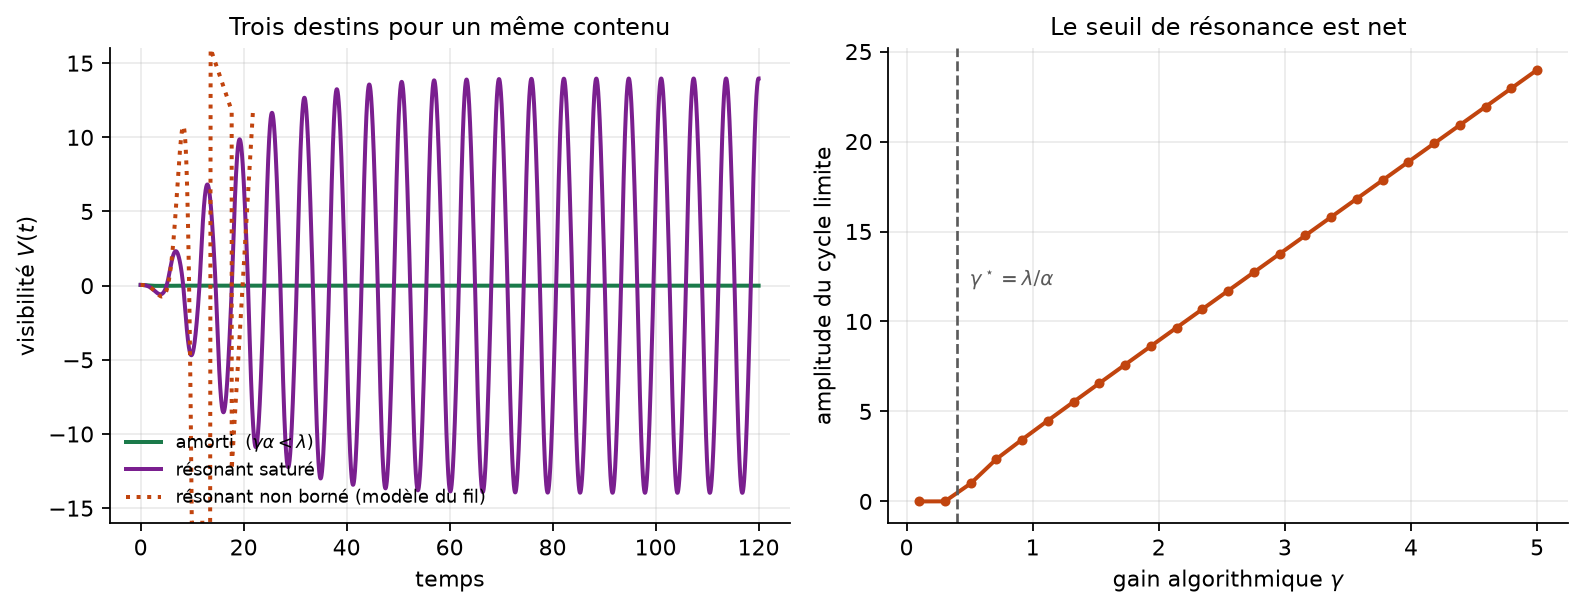
\includegraphics[width=\linewidth]{fig06_resonance.png}
\caption{À gauche, trois destins pour un même contenu : amorti, résonant borné, résonant
non borné. À droite, amplitude du cycle limite en fonction du gain algorithmique ; le seuil
mesuré coïncide avec $\gamma^\star = \lambda/\alpha$.}
\label{fig:resonance}
\end{figure}

Un point mérite d'être souligné pour la régulation. À gain \emph{uniforme}, un contenu plus
émotionnel franchit le seuil qu'un contenu factuel ne franchit pas. Une plateforme n'a donc
pas besoin de favoriser la désinformation pour l'amplifier sélectivement : le biais est
mécanique. C'est ce qui rend la mesure de $\gamma$ plus pertinente, et plus opposable,
qu'un audit d'intentions éditoriales.

\section{Deux instruments}

\subsection{L'Index de Dissipation Entropique}

L'IDE est l'entropie de Shannon des points de vue servis à un utilisateur, normalisée par
son maximum théorique :
\begin{equation}
\mathrm{IDE} = \frac{H(X)}{\log_2 k} \in [0,1].
\label{eq:ide}
\end{equation}
La normalisation est le point essentiel : elle rend l'index sans dimension et comparable
entre plateformes, ce qu'un seuil exprimé en bits ne permet pas. Le dénominateur $k$ --- le
nombre de points de vue que la plateforme est \emph{en mesure} de servir --- doit être
imposé par le régulateur, faute de quoi un fil parfaitement fermé obtiendrait un index
flatteur.

Un IDE effondré est la signature d'une température sociale locale nulle, c'est-à-dire d'un
état figé au sens du modèle d'Ising --- le régime dans lequel l'hystérésis rend les fausses
croyances persistantes.

\subsection{L'Algorithme de Dissipation Entropique}

Un algorithme de recommandation classique maximise l'engagement immédiat ; d'après
\eqref{eq:critere}, cette fonction de coût est celle qui produit l'amortissement négatif.
L'ADE la remplace par
\begin{equation}
S(i,c) = \mathrm{Pertinence}(i,c) + \mu \cdot \Delta H(i,c),
\qquad \mu \geq 0,
\label{eq:ade}
\end{equation}
où $\Delta H = H_{\mathrm{futur}} - H_{\mathrm{actuelle}}$ mesure l'impact du contenu sur
l'index du fil. Le signe positif est essentiel : il récompense la diversification. Le terme
de pertinence est conservé --- un algorithme servant de la diversité sans pertinence serait
abandonné par ses utilisateurs, ce qui ne dissiperait aucune entropie.

Le coefficient $\mu$ n'est pas constant. Il reste à une valeur de repos tant que l'index est
satisfaisant, et croît progressivement lorsque celui-ci descend sous le seuil critique :
c'est la transposition du recuit simulé, un pic de température ponctuel pour casser un état
figé, suivi d'un refroidissement. À $\mu = 0$, l'ADE est indiscernable d'un filtre
d'engagement, ce qui en fait un ajout paramétré plutôt qu'une refonte.

\section{Calibration empirique du rapport d'amplification}
\label{sec:calibration}

Le critère \eqref{eq:critere} est resté longtemps une inégalité formelle : rien n'indiquait
où se situent les systèmes réels. Nous l'estimons ici sur des séries d'attention publiques.

\subsection{Identification}

Pour un pic d'attention isolé, non oscillatoire, \eqref{eq:resonance} se réduit à sa forme
du premier ordre $\dot V = \gamma\alpha\,\sigma(V)V - \lambda V$, qui se sépare en deux
régimes mesurables : pendant la \emph{montée}, la saturation est inactive et
$V \propto e^{(\gamma\alpha-\lambda)t}$ ; pendant la \emph{décroissance}, l'amplification est
éteinte et $V \propto e^{-\lambda t}$. Deux régressions log-linéaires donnent donc
\begin{equation}
\lambda = r_{\mathrm{down}}, \qquad \gamma\alpha = r_{\mathrm{up}} + r_{\mathrm{down}},
\qquad \frac{\gamma\alpha}{\lambda} = 1 + \frac{r_{\mathrm{up}}}{r_{\mathrm{down}}}.
\label{eq:identification}
\end{equation}

\subsection{Données}

Les séries proviennent de l'API de consultations de Wikimedia, filtrées sur l'agent
\texttt{user} pour exclure les robots, sur un corpus de 24 sujets \emph{pré-enregistré} et
réparti en deux registres émotionnels — accusation ou scandale d'une part, découverte non
programmée d'autre part. Wikipédia étant dépourvue d'algorithme de recommandation, le
$\gamma$ ainsi estimé est un gain d'\emph{écosystème} et non la fonction de classement d'une
plateforme.

\subsection{Résultats}

Dix-neuf épisodes sont exploitables. Le rapport vaut entre $1{,}5$ et $12$, de médiane
$2{,}5$ à $4{,}2$ selon l'estimateur (figure~\ref{fig:calibration}). Trois enseignements,
dont deux négatifs.

\paragraph{Le critère de signe est vide.} Le rapport dépasse $1$ dans tous les épisodes et
sous tous les estimateurs. Ce n'est pas une propriété de l'écosystème mais une
\emph{tautologie de la procédure} : un épisode observable a nécessairement connu une phase de
croissance, donc $r_{\mathrm{up}} > 0$. La recommandation « interdire les configurations où
$\gamma\alpha > \lambda$ » est par conséquent inapplicable, et doit être remplacée par un
\textbf{plafond} $\gamma\alpha/\lambda \leq \rho_{\max}$. Cette erreur n'était pas
détectable par relecture : seule la tentative de mesure l'a révélée.

\paragraph{La valeur dépend de la méthode.} Avec des fenêtres délimitées par le retour au
niveau de fond, leur durée varie de 6 à 46 jours ; l'attention décroissant plus lentement
qu'une exponentielle, un ajustement sur une fenêtre longue produit un $\lambda$ plus faible.
La corrélation de rang atteint $-0{,}94$. Un second estimateur, à horizon fixe, rend
$\lambda$ comparable entre épisodes ; la médiane varie néanmoins d'un facteur $1{,}7$ selon
l'estimateur retenu, ce qui interdit d'adosser un seuil réglementaire à une valeur unique.

\paragraph{Le mécanisme de la charge émotionnelle n'est pas étayé.} Aucun écart détectable
entre les deux registres ($p \geq 0{,}13$), et l'estimation ponctuelle va dans le sens
contraire à la prédiction. Les effectifs sont faibles et le biais de sélection décrit
ci-dessous écarte les cas les plus chargés ; il serait donc excessif d'y voir une
réfutation — mais le mécanisme ne peut pas être présenté comme soutenu par les données.

\paragraph{La méthode est aveugle aux régimes installés.} Onze sujets sur vingt-quatre ne
livrent aucun épisode exploitable, et ce sont les cas archétypaux : QAnon, désinformation
sanitaire, hésitation vaccinale. Leur attention ne forme pas un pic mais un \emph{palier
durable}, que le niveau de fond glissant absorbe — la détection par proéminence ne les voit
pas. La procédure sélectionne donc contre le phénomène même que la théorie décrit, ce qui
constitue la limite la plus lourde de cette calibration.

\begin{figure}[t]
\centering
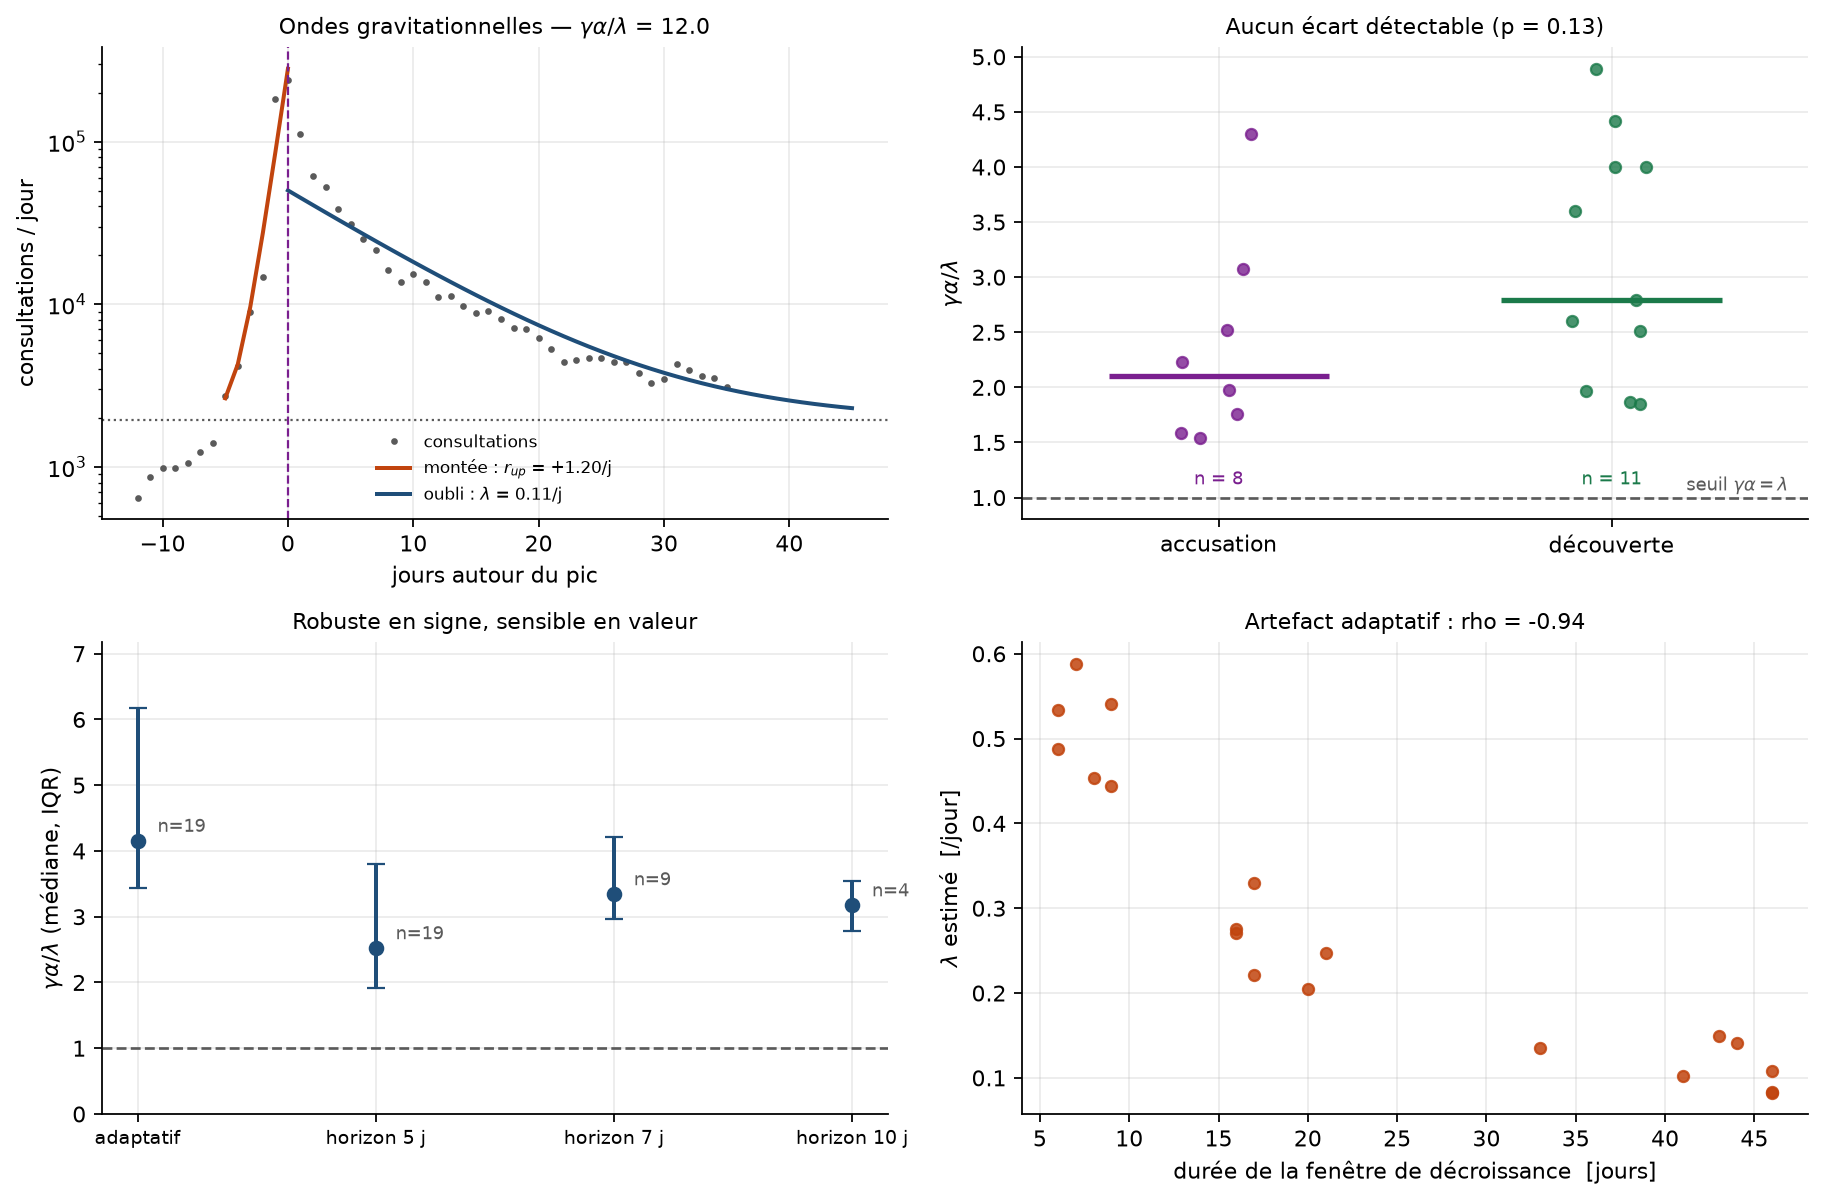
\includegraphics[width=\linewidth]{fig09_calibration.png}
\caption{Un épisode d'attention et ses deux régimes exponentiels ; la distribution du rapport
par registre émotionnel ; la sensibilité de la médiane au choix d'estimateur ; et l'artefact
de fenêtre qui a imposé l'estimateur à horizon fixe.}
\label{fig:calibration}
\end{figure}

\section{Limites}
\label{sec:limites}

Ces limites sont énoncées ici plutôt que laissées aux relecteurs.

\paragraph{Calibration empirique à peine entamée.} C'est la faiblesse principale. Un seul
paramètre composite est estimé (\S\ref{sec:calibration}) ; $J$, $T$, $\gamma$ et $\alpha$
pris séparément n'ont aucune procédure d'estimation. La voie la plus prometteuse serait
l'inférence des coefficients de Kramers-Moyal sur des séries d'opinion longues, qui
permettrait de \emph{tester} la dérive \eqref{eq:derive} plutôt que de l'ajuster.

\paragraph{Une analogie n'est pas une explication.} Rien ici ne démontre que les opinions
\emph{obéissent} à une mécanique statistique. Le travail établit qu'un formalisme emprunté
à la physique \emph{reproduit} certains comportements observés. La prédiction de Kramers
sur la dépendance en température du taux de basculement offrirait un test falsifiable ;
il n'a pas été mené.

\paragraph{Les individus ne sont pas des spins.} L'intentionnalité, l'ironie et
l'anticonformisme stratégique n'ont pas d'équivalent dans un modèle de spins. Les opinions
sont multidimensionnelles --- le modèle à agents emploie deux axes continus, ce qui atténue
le problème sans le résoudre \citep{deffuant2000}. Enfin, l'environnement n'est pas
passif : un algorithme optimise une fonction de coût, ce qui en fait un acteur stratégique
plutôt qu'un bain thermique. C'est le point le plus fragile de l'analogie, et c'est aussi
ce qui rend l'ADE concevable --- une fonction de coût peut être changée.

\paragraph{Limites propres à l'index comme instrument.} La discrétisation en points de vue
est un choix politique : qui définit les modalités définit l'index. L'index est
manipulable, une plateforme pouvant servir des contenus formellement divergents mais
substantiellement vides. Sa mesure sur des fils individuels soulève une question de vie
privée à laquelle ce travail ne répond pas. Enfin, imposer un plancher d'IDE est une
contrainte sur ce que les citoyens voient : c'est défendable, mais c'est une intervention
sur le débat public, et la présenter comme une simple mesure technique serait malhonnête.

\paragraph{Portée des simulations.} Les régimes explorés ont été choisis pour leur
lisibilité. Aucune étude systématique de sensibilité n'a été menée, les tailles de systèmes
sont modestes, et aucun résultat n'est comparé à des données réelles. Les conclusions sont
qualitatives : elles portent sur l'existence de régimes et le sens des dépendances, jamais
sur des valeurs numériques transposables.

\section{Reproductibilité}

L'intégralité du travail est disponible en accès libre, exécutable en conteneur, avec
$203$ tests automatisés. Les vérifications structurantes portent sur la température
critique d'Onsager \eqref{eq:onsager}, la conservation exacte de la masse de probabilité,
les exposants des lois d'échelle du temps de consensus, la positivité de l'aire du cycle
d'hystérésis sous $T_c$, et l'équivalence de l'ADE avec un filtre d'engagement à
$\mu = 0$. Chaque figure de cette note est régénérée par un notebook.

\begin{center}
\url{https://github.com/s-geffroy/Index-Dissipation-Entropique}\\
\url{https://s-geffroy.github.io/Index-Dissipation-Entropique/}
\end{center}

Ce travail est ouvert à la relecture critique. Les retours portant sur la calibration
empirique, sur la viabilité de l'index comme instrument réglementaire, ou sur les analogies
restantes qui ne tiendraient pas, sont les plus utiles.

\bibliography{refs}

\end{document}
